Two of the central concepts in machine learning are \textbf{underfitting} and \textbf{overfitting}.\cite{goodfellow_deep_2016} Underfitting occurs when a model is unable to achieve sufficiently low error even on the training set. This usually indicates that the model is too simple, insufficiently trained, or poorly configured for the complexity of the task. Overfitting, by contrast, occurs when the model performs very well on the training data but poorly on unseen data, meaning that it has adapted too strongly to idiosyncrasies of the training set rather than learning patterns that generalize.\cite{goodfellow_deep_2016}
\begin{figure}[ht]
    \centering
    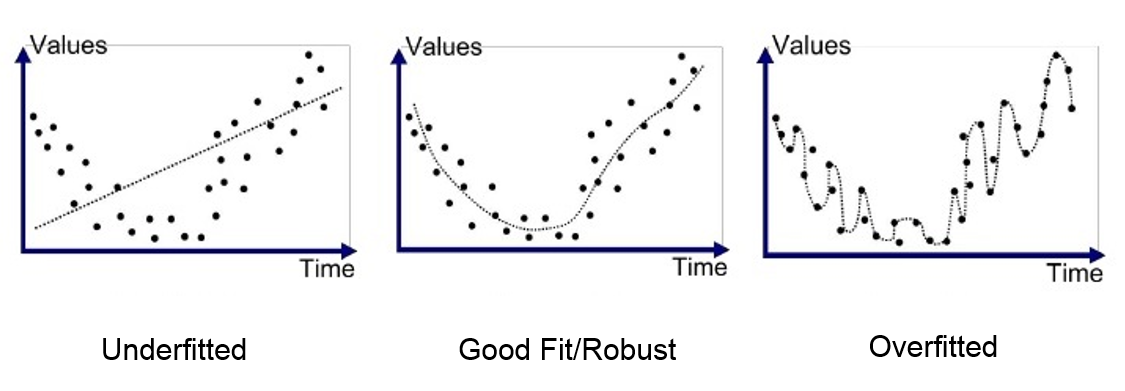
\includegraphics[width=0.75\linewidth]{images/under_over_example.png}
    \caption{Example of underfitting and overfitting in a regression task. The left plot shows an underfitting model that fails to capture the underlying trend, the middle plot shows a well-fitted model that generalizes well, and the right plot shows an overfitting model that captures noise in the training data.}
    \label{fig:example_under_overfitting}
\end{figure}

These two phenomena can often be identified through the evolution of training and validation curves. In an underfitting regime, both training and validation errors remain relatively high. In an overfitting regime, the training error keeps decreasing whereas the validation error stagnates or starts increasing. Monitoring these trends is therefore essential for understanding whether additional training is beneficial or detrimental.\cite{goodfellow_deep_2016,prechelt_early_2012}

One of the most widely used strategies for limiting overfitting is \textbf{early stopping}. During optimization, the training loss may continue to decrease even after the model has already reached its best generalization performance. When the validation error stops improving and begins to worsen, this is a signal that the model is starting to adapt too closely to the training data. Early stopping addresses this issue by interrupting training at the point of best validation performance and retaining the corresponding model parameters.\cite{goodfellow_deep_2016,prechelt_early_2012}
\begin{figure}[ht]
    \centering
    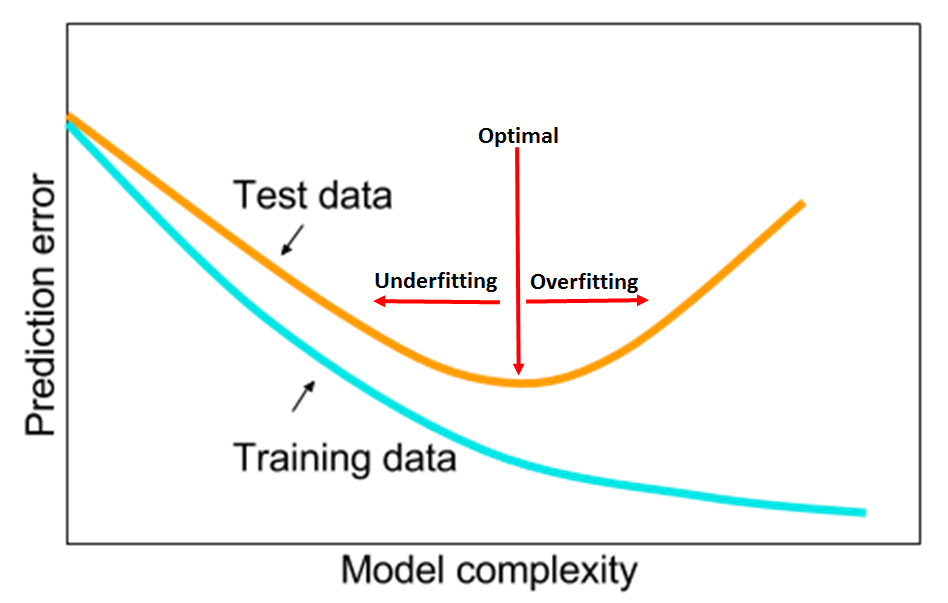
\includegraphics[width=0.6\linewidth]{images/under-overfitting.png}
    \caption{Typical training and validation behaviors in underfitting and overfitting regimes.}
    \label{fig:learning_curves_overfitting}
\end{figure}

Several strategies can be adopted to mitigate these problems. Underfitting may be addressed by increasing model capacity, improving feature quality, extending training, or refining optimization settings. Overfitting can instead be reduced through regularization techniques, data augmentation, early stopping, or, when appropriate, by simplifying the model.\cite{goodfellow_deep_2016} In practice, achieving good generalization requires balancing model capacity and training duration so that the model captures meaningful structure in the data without memorizing the training set.
